
\documentclass[12pt]{article}
%\usepackage[finnish]{babel}
\usepackage[T1]{fontenc}
\usepackage[utf8]{inputenc}
\usepackage{amssymb}
\usepackage{amsmath}
\usepackage{graphicx}
\usepackage{hyperref}
\usepackage{mathtools}


\newcommand{\pat}{\partial}
\newcommand{\be}{\begin{equation}}
\newcommand{\ee}{\end{equation}}
\newcommand{\bea}{\begin{eqnarray}}
\newcommand{\eea}{\end{eqnarray}}
\newcommand{\abf}{{\bf a}}
\newcommand{\Zcal}{{\cal Z}_{12}}
\newcommand{\zcal}{z_{12}}
\newcommand{\Acal}{{\cal A}}
\newcommand{\Fcal}{{\cal F}}
\newcommand{\Ucal}{{\cal U}}
\newcommand{\Vcal}{{\cal V}}
\newcommand{\Ocal}{{\cal O}}
\newcommand{\Rcal}{{\cal R}}
\newcommand{\Scal}{{\cal S}}
\newcommand{\Lcal}{{\cal L}}
\newcommand{\Hcal}{{\cal H}}
\newcommand{\hsf}{{\sf h}}
\newcommand{\half}{\frac{1}{2}}
\newcommand{\Xbar}{\bar{X}}
\newcommand{\xibar}{\bar{\xi }}
\newcommand{\barh}{\bar{h}}
\newcommand{\Ubar}{\bar{\cal U}}
\newcommand{\Vbar}{\bar{\cal V}}
\newcommand{\Fbar}{\bar{F}}
\newcommand{\zbar}{\bar{z}}
\newcommand{\wbar}{\bar{w}}
\newcommand{\zbarhat}{\hat{\bar{z}}}
\newcommand{\wbarhat}{\hat{\bar{w}}}
\newcommand{\wbartilde}{\tilde{\bar{w}}}
\newcommand{\barone}{\bar{1}}
\newcommand{\bartwo}{\bar{2}}
\newcommand{\nbyn}{N \times N}
\newcommand{\repres}{\leftrightarrow}
\newcommand{\Tr}{{\rm Tr}}
\newcommand{\tr}{{\rm tr}}
\newcommand{\ninfty}{N \rightarrow \infty}
\newcommand{\unitk}{{\bf 1}_k}
\newcommand{\unitm}{{\bf 1}}
\newcommand{\zerom}{{\bf 0}}
\newcommand{\unittwo}{{\bf 1}_2}
\newcommand{\holo}{{\cal U}}
%\newcommand{\bra}{\langle}
%\newcommand{\ket}{\rangle}
\newcommand{\muhat}{\hat{\mu}}
\newcommand{\nuhat}{\hat{\nu}}
\newcommand{\rhat}{\hat{r}}
\newcommand{\phat}{\hat{\phi}}
\newcommand{\that}{\hat{t}}
\newcommand{\shat}{\hat{s}}
\newcommand{\zhat}{\hat{z}}
\newcommand{\what}{\hat{w}}
\newcommand{\sgamma}{\sqrt{\gamma}}
\newcommand{\bfE}{{\bf E}}
\newcommand{\bfB}{{\bf B}}
\newcommand{\bfM}{{\bf M}}
\newcommand{\cl} {\cal l}
\newcommand{\ctilde}{\tilde{\chi}}
\newcommand{\ttilde}{\tilde{t}}
\newcommand{\ptilde}{\tilde{\phi}}
\newcommand{\utilde}{\tilde{u}}
\newcommand{\vtilde}{\tilde{v}}
\newcommand{\wtilde}{\tilde{w}}
\newcommand{\ztilde}{\tilde{z}}
\newcommand{\ket}[1]{\vert{#1}\rangle}
\newcommand{\bra}[1]{\langle{#1}\vert}

\usepackage{listings}
\DeclarePairedDelimiter\abs{\lvert}{\rvert}%
\DeclarePairedDelimiter\norm{\lVert}{\rVert}%

% Swap the definition of \abs* and \norm*, so that \abs
% and \norm resizes the size of the brackets, and the 
% starred version does not.
\makeatletter
\let\oldabs\abs
\def\abs{\@ifstar{\oldabs}{\oldabs*}}
%
\let\oldnorm\norm
\def\norm{\@ifstar{\oldnorm}{\oldnorm*}}
\makeatother

\hoffset 0.5cm
\voffset -0.4cm
\evensidemargin -0.2in
\oddsidemargin -0.2in
\topmargin -0.2in
\textwidth 6.3in
\textheight 8.4in

\begin{document}

\normalsize

\baselineskip 14pt

\begin{center}
{\Large {\bf Numerical Methods in Scientific Computing 2021 \ \ \\ Answers Ex02}} \\
Jake Muff
29/01/21
\end{center}
\section*{Problem 1}
Show that for a vector $\vec{x}$ of length $n$ 
$$ \lim{p \to \infty} \Big[ \sum_{i=1}^n \abs{ x_i} ^p \Big]^{\frac{1}{p}} = \text{max}_{i \leq i \leq n} (\abs{ x_i} )  $$
To show this lets denote $x_j$ to be the largest element in the vector so that 
$$ \lim{p \to \infty} \Big[ \sum_{i=1}^n \abs{x_i}^p \Big]^{\frac{1}{p}} = \lim_{p \to \infty} \Big[ \abs{ x_1}^p + \abs{x_2}^p + \ldots \abs{ x_j}^p + \ldots \abs{ x_n}^p \Big]^{\frac{1}{p}} $$
If we factor $x_j$ out 
$$ = x_j \Big[ \lim_{p \to \infty} \Big[ \abs{\frac{x_1}{x_j}}^p + \abs{\frac{x_2}{x_j}}^p + \ldots 1 + \ldots \abs{\frac{x_n}{x_j}}^p \Big] ^{\frac{1}{p}} \Big] $$
Because $x_j$ is defined as the largest vector, 
$$ \frac{x_i}{x_j} < 1 $$
Thus 
$$ \abs{\frac{x_i}{x_j} }^p \rightarrow 0 \ \text{as} \ p \rightarrow \infty $$
This means that
\begin{equation}
\Big[ \abs{\frac{x_1}{x_j} }^p + \abs{\frac{x_2}{x_j} }^p + \ldots 1 + \ldots \abs{\frac{x_n}{x_j} }^p \Big]^{\frac{1}{p} } \rightarrow 0^0 \ \text{as} \ p \rightarrow \infty 
\end{equation} 
Mostly $0^0$ is defined as $1$ but it can be undefined/indeterminant and the limit can be found using L'Hôpital's rule, which uses the derivative to evaluate the limit. So, for example, we have 
$$ a = \Big( \frac{1}{b} \Big)^{\frac{1}{b} } $$
$$ \lim_{b \to \infty} a = 0^0 $$
To use L'Hôpital's rule we need it in the form $\frac{f(b)}{g(b)}$. Thus,
$$ \ln a = \frac{1}{b} \ln \frac{1}{b} = - \frac{\ln b}{b}  $$
$$ \lim_{b \to \infty} \ln a = - \lim_{b \to \infty} \frac{\ln b}{b} = \frac{f(b)}{g(b)} $$
$$ \frac{f'(b)}{g'(b)} = \frac{\frac{1}{b}}{1} $$
$$ - \lim_{b \to \infty} \frac{\ln b}{b} = - \lim_{b \to \infty} \frac{\frac{1}{b}}{1} $$
Which can be evaluated 
$$ \lim_{b \to \infty} \ln a = 0 $$
Such that 
$$ \lim_{b \to \infty} a = e^{\lim_{b \to \infty} \ln a} = 1 $$
Thus 
$$ \lim_{b \to \infty} \Big( \frac{1}{b} \Big)^{\frac{1}{b}} = 1 $$
Applying this to equation (1)
$$ \lim_{p \to \infty} \Big[ \abs{\frac{x_1}{x_j} }^p + \abs{\frac{x_2}{x_j} }^p + \ldots 1 + \ldots \abs{\frac{x_n}{x_j} }^p \Big]^{\frac{1}{p} } = 1 $$
Thus 
$$ \lim{p \to \infty} \Big[ \sum_{i=1}^n \abs{ x_i} ^p \Big]^{\frac{1}{p}} = x_j \cdot \Big[ \lim_{p \to \infty} \Big[ \abs{\frac{x_1}{x_j} }^p + \abs{\frac{x_2}{x_j} }^p + \ldots 1 + \ldots \abs{\frac{x_n}{x_j} }^p \Big]^{\frac{1}{p} } \Big] $$
$$ = x_j \cdot 1 $$
$$ = x_j $$
And $x_j$ is defined as the max element, so, 
$$ = \text{max}_{i \leq i \leq n} (\abs{ x_i} )  $$


\section*{Problem 2}
In this problem I had to implement the Kahan summation algorithm into the previous weeks 
work. The source file for this question is found under \lstinline{harmonc_kahan.cpp}.
The results are shown below. The function correctly returns the sum of the first N terms. Compared to the previous week it is interesting to note that at the same value (2097152) the function does not converge to a single finite value. Instead, as shown
it prints finite values for numbers significantly higher than what was used in the previous week but still not infinite. This tells me that this algorithm is more precise and 'better' than the previous weeks 
but still not ideal as it converges to a finite value. 

\begin{figure}
    
    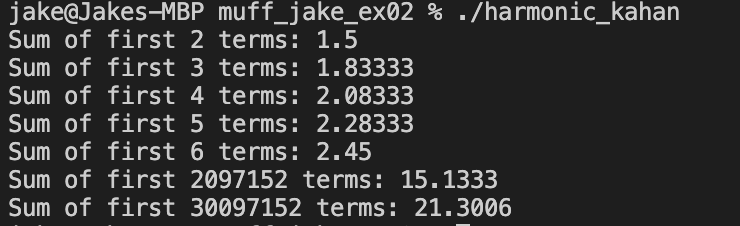
\includegraphics[width=10cm]{harmonc_kahan.png}
    \centering
    \caption{Output from \lstinline{harmonic_kahan.cpp}}

\end{figure}

\section*{Problem 3}
Despite being a seemingly simple problem, it took a surprising amount of time due to trying to get LAPACK to work on my computer. For this I used LAPACK on OSX Catalina 31/1/21
Since OSX Mavericks there is a system install version of LAPACK and BLAS that is optimized for use on OSX devices but often requires use of XCODE or fiddling about with default path locations.
Another method is to use Homebrew with \\
\\
\lstinline{brew install lapack (or Lapack)} \\
\\
Which installs LAPACK as well as BLAS and dependencies. To use this in compilation requires addition of \lstinline{-L/Path/To/Directory} which is usually in \lstinline{/usr/local/lib}
In the end I used A.Kuronen version of LAPACK from SC II example Progs page which requires compiling 
using gfortran after you have read the README file attached \\
\\
\lstinline{gfortran -o ex2_p3 ex2_p3.c -llapack} \\
\\
NOTE: There is a implicit declaration warning due to calling the LAPACK function but not declaring in a header file as requires in C99. Can still rule the executable. This method just outdated imo but still works. \\
NOTE: The lineardouble and eigendouble files in the .tar from Example Progs Page are terribly commented and coded for use of Matrices and general linear algebra, therefore, I edited them by adding in input from file and printf statements \\
\\

\begin{figure}
    
    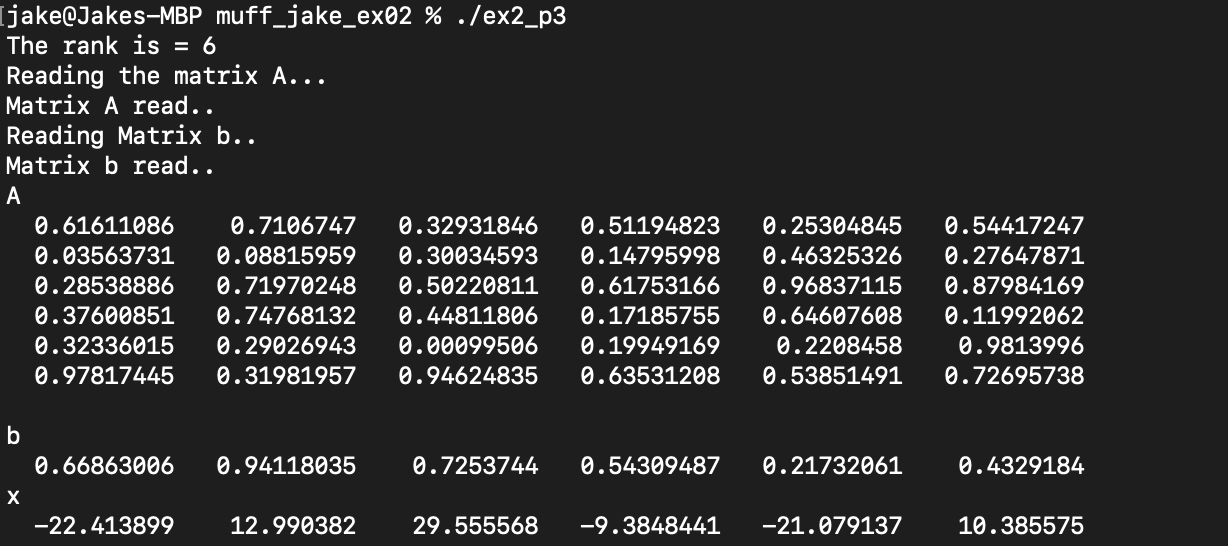
\includegraphics[width=10cm]{matrix6.png}
    \centering
    \caption{Output from \lstinline{ex2_p3.c}, solving matrix6 for the vector x. }

\end{figure}

\begin{figure}
    
    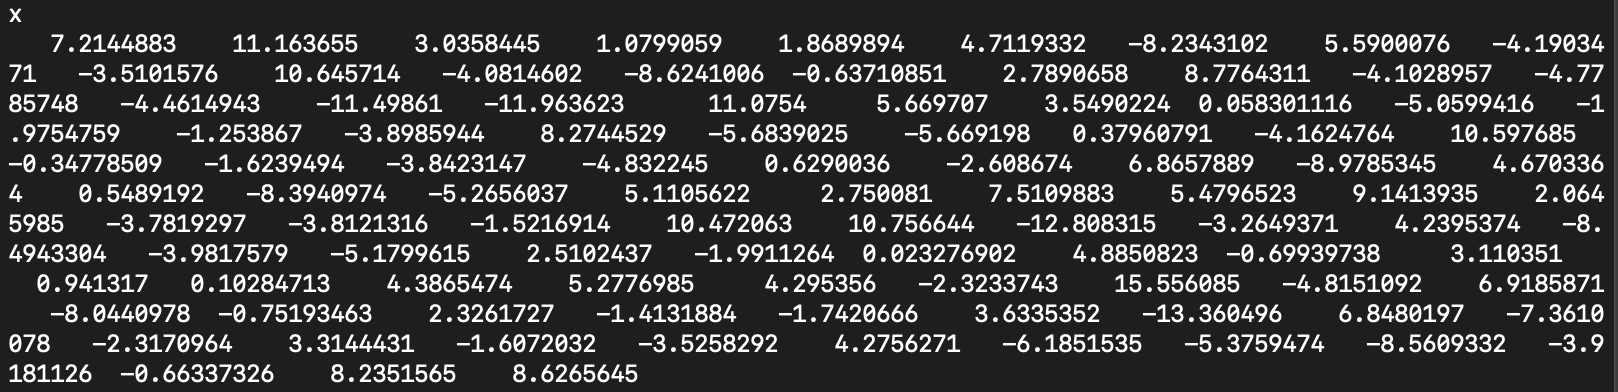
\includegraphics[width=10cm]{matrix100.png}
    \centering
    \caption{Output from \lstinline{ex2_p3.c}, solving matrix100 for the vector x. Obviously due to the size of the matrix, the output is messy but the solution should be correct. }

\end{figure}

For Part B, "edit matrix6 in such a way that it becomes singular" I did not fully understand. A singular matrix has determinant 0 and is therefore non-invertible. To make matrix6 singular, the easiest way would just to make matrix6 entirely 0's, however I do not think this is what you mean in this question.
I am not quite sure by what method you wish us to make it singular. The closest idea I came up with was to REF the matrix and change the diagonal value to a 0 thereby making the determinant 0. 


\section*{Problem 4} 
For this problem I first copied over the problem 3 code into the function to get the vector $\vec{x}$. Then I used the LAPACK subroutine \lstinline{dgemm} to multiple the Matrix $A$ and the vector $\vec{x}$, the subroutine also allows for $\vec{b}$ to be taken away. 
The only problem arose when doing this was the fact that because the subroutine is written in fortran it only takes pointers as inputs. 
I then calculated the norm below it by using an IF statement as well as FOR loops. 
\\
I implemented 
$$ \Big( \sum_{i=1}^n |x_i|^m \Big)^{\frac{1}{m}} $$
For $m=1,2 \ldots$. For $m = 0$ in the loop, the IF statement calls it and calculates the max absolute value in the vector according to the infinity norm. 

\begin{figure}
    
    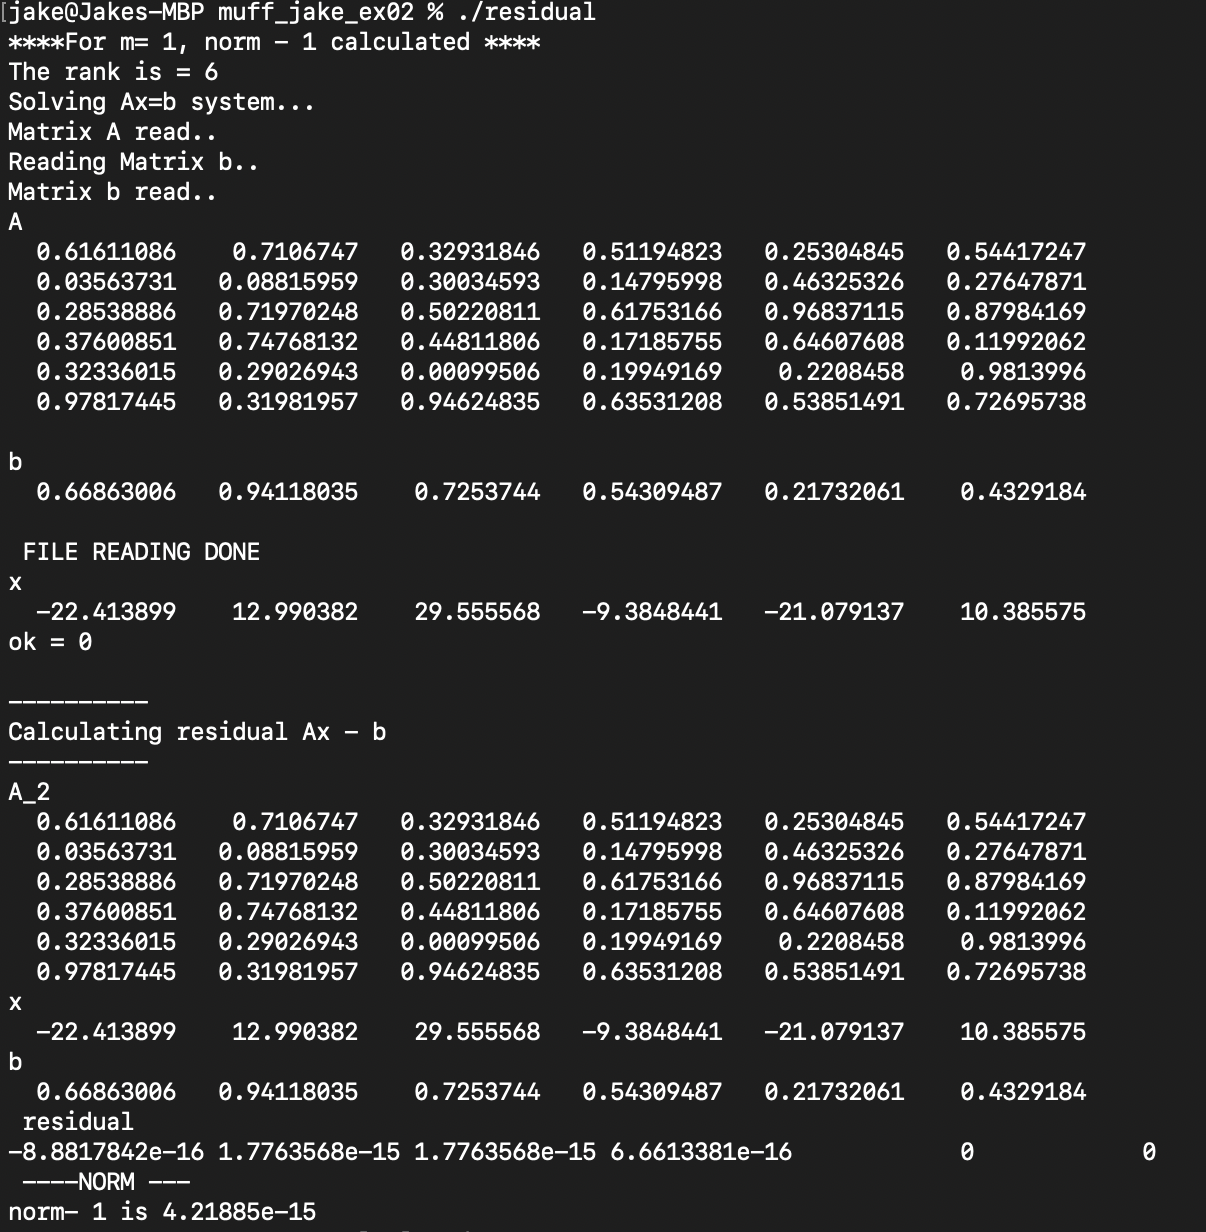
\includegraphics[width=10cm]{norm1.png}
    \centering
    \caption{Output from \lstinline{residual.c} for $m=1$.}

\end{figure}

\begin{figure}
    
    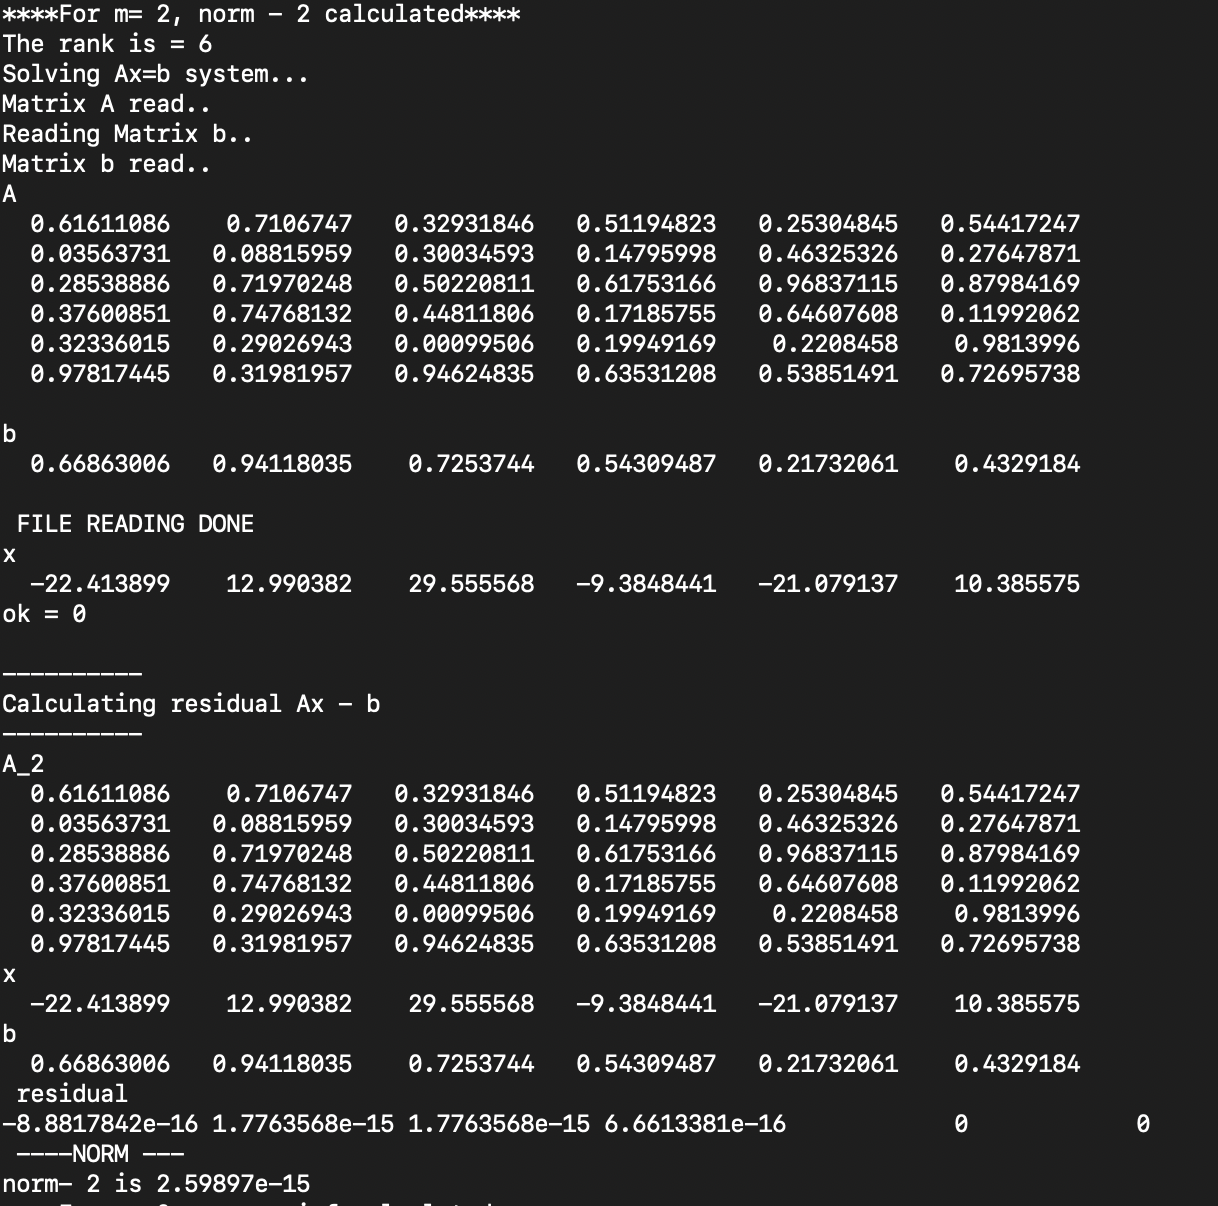
\includegraphics[width=10cm]{norm2.png}
    \centering
    \caption{Output from \lstinline{residual.c} for $m=2$.}

\end{figure}

\begin{figure}
    
    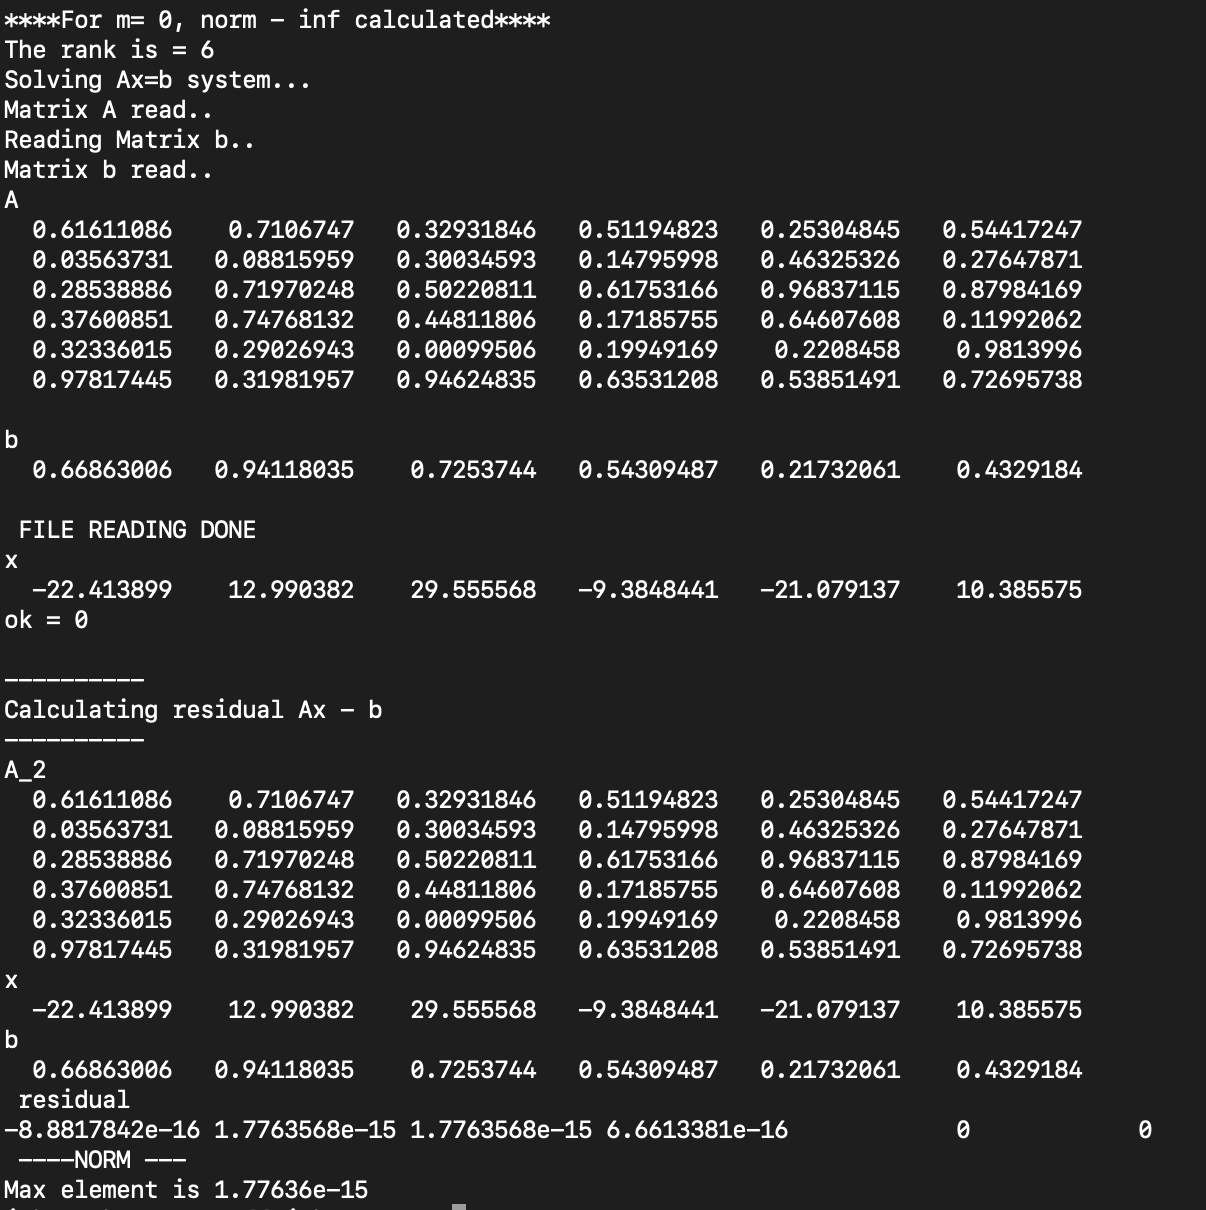
\includegraphics[width=10cm]{norminf.png}
    \centering
    \caption{Output from \lstinline{residual.c} for $m= \infty$.}

\end{figure}

\end{document}


